\documentclass[a4paper]{article}

\usepackage[UTF8]{ctex}
\usepackage[a4paper,margin=1in]{geometry}
\usepackage{graphicx}
\usepackage{float}
\usepackage{listings}
\usepackage{longtable}
\usepackage{booktabs}
\usepackage{hyperref}
\usepackage{fancyhdr}
\usepackage{lastpage}
\usepackage{color}
\usepackage{indentfirst}        % 首段缩进
\setlength{\parindent}{2em}     % 缩进2字符
\usepackage{zhnumber}           % 中文编号
\usepackage[dvipsnames]{xcolor}

%\newcommand{\college}{中山大学计算机学院}
\newcommand{\projname}{数据库系统原理实验|实验九}
\newcommand{\reporttitle}{ER图的绘制}
\newcommand{\stuno}{23336179}
\newcommand{\authorname}{马福泉}
\newcommand{\major}{计算机科学与技术}
\newcommand{\adviser}{赖韩江}
\newcommand{\startdate}{2025年11月20日}
\newcommand{\labenddate}{2025年11月27日}
\newcommand{\labroom}{B202}

\pagestyle{fancy} % 使用 fancyhdr 风格
\fancyhf{}      % 清空默认的页眉页脚

% 设置页眉
\fancyhead[L]{\kaishu \projname}      % 左侧页眉显示项目名称
\fancyhead[C]{\kaishu \reporttitle}    % 中间页眉显示报告标题
\fancyhead[R]{\kaishu \authorname} % 右侧页眉显示作者姓名

% 设置页脚
\fancyfoot[C]{第 \thepage 页，共 \pageref{LastPage} 页} % 中间页脚显示页码

% 去除页眉页脚与正文之间的分隔线
\renewcommand{\headrulewidth}{0.4pt}
\renewcommand{\footrulewidth}{0pt}

% 设置文档背景颜色
\definecolor{mybgcolor}{RGB}{0, 0, 0} % 定义背景颜色
\definecolor{NavyBlue}{RGB}{0,0,128} % 添加颜色定义
% \pagecolor{mybgcolor} % 设置背景颜色

% listing 配置rust
% \lstdefinelanguage{Rust}{
%   keywords={fn, let, mut, struct, enum, impl, pub, use, mod, trait, where},
%   keywordstyle=\color{NavyBlue},
%   comment=[l]{//},
%   commentstyle=\color{gray},
% }
% \lstset{language=Rust}

\lstset{
  basicstyle=\ttfamily\small,
  keywordstyle=\color{NavyBlue},
  commentstyle=\color{gray},
  stringstyle=\color{red},
  showstringspaces=false,
  extendedchars=false, % 关键：不处理中文
  breaklines=true,
  language=Python
}

\begin{document}

% 封面
\begin{titlepage}
    \centering
    
\includegraphics[width=10cm]{img/SYSULogo.png}

    \vspace{1em}
    %{\Large \college \par}
    \vspace{1em}
    {\Large \kaishu \projname \par}
    \vspace{3em}

    

    
    {\fontsize{40pt}{42pt}\kaishu \selectfont \boldmath \reporttitle\par}
    \vspace*{\fill}

    \begin{center}
    {\Large
    \makebox[5em][s]{学号}:\underline{\makebox[15em][c]{\kaishu \stuno}}\\[1em]
    \makebox[5em][s]{姓名}:\underline{\makebox[15em][c]{\kaishu \authorname}}\\[1em]
    \makebox[5em][s]{专业}:\underline{\makebox[15em][c]{\kaishu \major}}\\[1em]
    \makebox[5em][s]{课程教师}:\underline{\makebox[15em][c]{\kaishu \adviser}}\\[1em]
    \makebox[5em][s]{起始日期}:\underline{\makebox[15em][c]{\kaishu \startdate}}\\[1em]
    \makebox[5em][s]{结束日期}:\underline{\makebox[15em][c]{\kaishu \labenddate}}\\[1em]
    \makebox[5em][s]{实验地点}:\underline{\makebox[15em][c]{\kaishu \labroom}}
    }
    \end{center}

    \vspace*{\fill}
\end{titlepage}

% 目录
\tableofcontents
\newpage

\section{实验概述}

1．数据库设计\\
为某电影院设计数据库。每部电影需记录名字、主演、导演、发行公司信息。一部电影上映多个场次，场次要记录播放时间，影厅号，影厅类型（IMAX，杜比、普通厅等）、原票价。每个场次售出多张电影票，电影票要记录座位号、实际票价。影院设有会员制，一个会员可购买多张电影票，会员要记录会员卡号，姓名，联系方式，充值记录。\\
（1）根据上述语义画出E-R图。\\
（2）将该E-R模型转换为关系模型。\\
2. 为实验教材上的 school 数据库画E-R图。

\section{实验报告}

\subsection{电影院数据库设计}

\subsubsection{E-R图}
\begin{figure}[H]
    \centering
    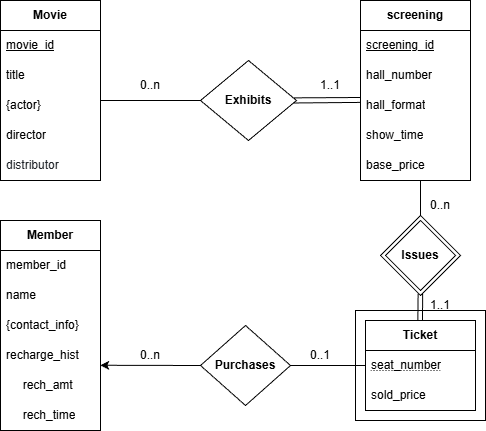
\includegraphics[width=0.9\textwidth]{img/cinema.png}
    \caption{电影院数据库E-R图}
\end{figure}

\subsubsection{实体（Entity）的设计与属性}
图中包含四个主要实体，分别对应现实世界中的四个核心对象：

\begin{enumerate}
    \item \textbf{Movie（电影）：}
    \begin{itemize}
        \item \textbf{性质：} 强实体。
        \item \textbf{属性：} 选取 \texttt{movie\_id} 作为主键（Primary Key，下划线标出）唯一标识一部电影。\texttt{title}（电影名）、\texttt{director}（导演）、\texttt{distributor}（发行公司）为普通单值属性。
        \item \textbf{特殊属性：} \texttt{\{actor\}} 被设计为多值属性（Multivalued Attribute），用花括号 \{\} 标记。这对应需求中“一部电影有多个主演”的语义。
    \end{itemize}

    \item \textbf{Screening（场次）：}
    \begin{itemize}
        \item \textbf{性质：} 强实体（引入代理键优化）。
        \item \textbf{属性：} \texttt{screening\_id}（主键）、\texttt{show\_time}、\texttt{hall\_number}、\texttt{hall\_format}、\texttt{base\_price}。
        \item \textbf{设计说明（为什么要加 ID？）：}
        \begin{itemize}
            \item \textbf{主键臃肿问题：} 如果 Screening 是弱实体，它的主键将是复合主键（如 Movie\_ID + Show\_Time + Hall\_Number）。
            \item \textbf{连锁反应：} Ticket 也是弱实体，依赖于 Screening。如果 Screening 没有独立 ID，Ticket 的主键将变成：Movie\_ID + Show\_Time + Hall\_Number + Seat\_Number。一张电影票表的主键包含4个字段，会导致查询慢、索引大、外键关联麻烦。
            \item \textbf{引入代理键 (Surrogate Key)：} 因此，“人为”引入了 \texttt{screening\_id} 作为代理主键，使其成为强实体，便于管理和引用。
        \end{itemize}
    \end{itemize}

    \item \textbf{Member（会员）：}
    \begin{itemize}
        \item \textbf{性质：} 强实体。
        \item \textbf{属性：} \texttt{member\_id} 为主键。\texttt{\{contact\_info\}} 为多值属性，表示会员可能有多个联系方式。
        \item \textbf{复合属性：} \texttt{recharge\_hist}（充值记录）包含 \texttt{rech\_amt}（金额）和 \texttt{rech\_time}（时间）。在概念模型中，这表示会员包含充值历史信息。
    \end{itemize}

    \item \textbf{Ticket（电影票）：}
    \begin{itemize}
        \item \textbf{性质：} 弱实体（Weak Entity）。
        \item \textbf{画法解释：} 使用双边框矩形表示。
        \item \textbf{理由：} 电影票的“座位号”在整个影院系统中不是唯一的（不同场次都有1排1座）。电影票必须依赖于具体的“场次”才能存在。因此，它没有完整的主键。
        \item \textbf{属性：} \texttt{seat\_number} 下方画了虚线，表示它是部分键（Partial Key）或分辨符。它只能在某一个特定的场次中区分不同的票。
    \end{itemize}
\end{enumerate}

\subsubsection{关系（Relationship）及其约束}
图中通过菱形框表示实体间的联系，具体的基数比（Cardinality）和参与度（Participation）解释如下：

\begin{enumerate}
    \item \textbf{Exhibits（放映）关系}
    \begin{itemize}
        \item \textbf{连接实体：} Movie 与 Screening
        \item \textbf{语义：} 一部电影被安排在多个场次放映。
        \item \textbf{基数约束 (0..n : 1..1)：}
        \begin{itemize}
            \item \textbf{Movie端 (0..n)：} 一部电影可以对应 0 个或 n 个场次（一对多关系）。0 表示电影已录入系统但尚未排片。
            \item \textbf{Screening端 (1..1)：} 一个场次必须且只能放映一部电影。
        \end{itemize}
        \item \textbf{双线（Double Line）含义：} Screening 侧使用了双线连接菱形，表示全参与（Total Participation）。即：不存在“没有电影”的空白场次，任何一个场次实体的存在，都必须依附于一部电影。
    \end{itemize}

    \item \textbf{Issues（出票/包含）关系 —— 弱实体联系}
    \begin{itemize}
        \item \textbf{连接实体：} Screening 与 Ticket
        \item \textbf{画法解释：} 使用双边框菱形。
        \item \textbf{含义：} 这是识别性关系（Identifying Relationship）。它专门用于连接弱实体（Ticket）和它的标识实体（Screening）。弱实体必须通过这个关系来确定身份。
        \item \textbf{基数约束 (0..n : 1..1)：}
        \begin{itemize}
            \item \textbf{Screening端 (0..n)：} 一个场次包含多张电影票（座位）。
            \item \textbf{Ticket端 (1..1)：} 一张电影票必须归属于一个特定的场次。
        \end{itemize}
        \item \textbf{双线含义：} Ticket 侧为双线，表示 Ticket 对该关系是全参与的。一张票脱离了场次就没有意义。
    \end{itemize}

    \item \textbf{Purchases（购买）关系}
    \begin{itemize}
        \item \textbf{连接实体：} Member 与 Ticket
        \item \textbf{语义：} 会员购买电影票。
        \item \textbf{基数约束 (0..n : 0..1)：}
        \begin{itemize}
            \item \textbf{Member端 (0..n)：} 需求指出“一个会员可购买多张电影票”，所以是 n。0 表示会员注册后可以暂时不买票。
            \item \textbf{Ticket端 (0..1)：} 一张具体的电影票，或者属于某一个会员（1），或者不属于任何会员（0）。
        \end{itemize}
        \item \textbf{关于0..1的解释：} 这里的 0 涵盖了两种情况：一是票还未售出；二是票被非会员（散客）购买，未关联到会员ID。这符合实际业务逻辑。
    \end{itemize}

\end{enumerate}

\subsubsection{关系模型转换}
将 E-R 图转换为关系模型（即数据库表结构），遵循以下规则：
\begin{itemize}
    \item \textbf{强实体}转为独立的表。
    \item \textbf{弱实体}转为独立的表，但必须包含父实体的主键作为外键。
    \item \textbf{1:n 关系}：将“1”端的主键加入到“n”端的表中作为外键。
    \item \textbf{多值属性}（如 \{actor\}）：必须单独拆分成一张新表。
\end{itemize}

基于上述规则，转换得到的最终关系模式如下（如图 \ref{fig:relation_model} 所示）：

\begin{figure}[H]
    \centering
    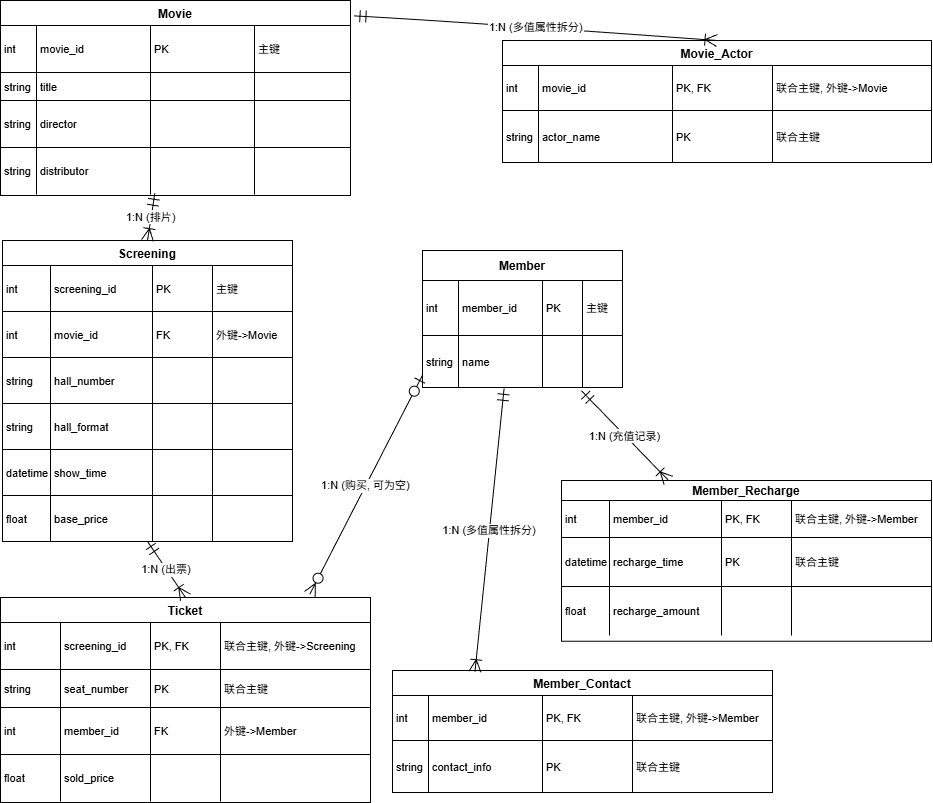
\includegraphics[width=0.9\textwidth]{img/relation_model..png}
    \caption{关系模型转换示意图}
    \label{fig:relation_model}
\end{figure}

\paragraph{1. 基础实体转换}
\begin{itemize}
    \item \textbf{Movie (电影表)}: Movie(\underline{movie\_id}, title, director, distributor)
    \item \textbf{Member (会员表)}: Member(\underline{member\_id}, name)
\end{itemize}

\paragraph{2. 处理多值/复合属性（拆分为新表）}
\begin{itemize}
    \item \textbf{Movie\_Actor (电影主演表)}: Movie\_Actor(\underline{movie\_id, actor\_name}) \\
    外键：\textit{movie\_id} 引用 Movie(movie\_id)
    \item \textbf{Member\_Contact (会员联系方式表)}: Member\_Contact(\underline{member\_id, contact\_info}) \\
    外键：\textit{member\_id} 引用 Member(member\_id)
    \item \textbf{Member\_Recharge (会员充值记录表)}: Member\_Recharge(\underline{member\_id, recharge\_time}, recharge\_amount) \\
    外键：\textit{member\_id} 引用 Member(member\_id)
\end{itemize}

\paragraph{3. 处理关系与外键}
\begin{itemize}
    \item \textbf{Screening (场次表)}: Screening(\underline{screening\_id}, hall\_number, hall\_format, show\_time, base\_price, \textit{movie\_id}) \\
    外键：\textit{movie\_id} 引用 Movie(movie\_id)
    \item \textbf{Ticket (电影票表)}: Ticket(\underline{screening\_id, seat\_number}, sold\_price, \textit{member\_id}) \\
    外键：\textit{screening\_id} 引用 Screening(screening\_id) \\
    外键：\textit{member\_id} 引用 Member(member\_id)
\end{itemize}

\subsection{School 数据库设计}

\subsubsection{E-R图}
\begin{figure}[H]
    \centering
    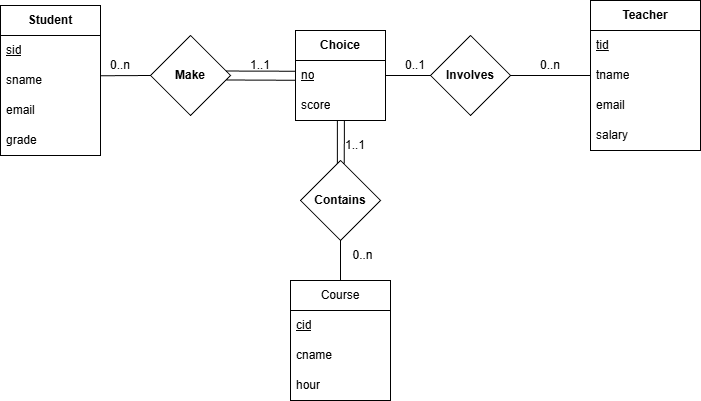
\includegraphics[width=0.9\textwidth]{img/school.png}
    \caption{School 数据库 E-R 图}
\end{figure}

\subsubsection{E-R图设计说明}
以下内容为系统概念模型设计说明。

\paragraph{A. 实体 (Entities) 的定义}
本系统包含四个强实体（Strong Entities），它们在图中均用普通矩形框表示，因为它们都拥有独立的、唯一的主键标识。

\begin{itemize}
    \item \textbf{Student (学生):} 主键为 \texttt{sid}，拥有属性 \texttt{sname} (姓名), \texttt{email} (邮箱), \texttt{grade} (年级)。
    \item \textbf{Teacher (教师):} 主键为 \texttt{tid}，拥有属性 \texttt{tname} (姓名), \texttt{email} (邮箱), \texttt{salary} (薪水)。
    \item \textbf{Course (课程):} 主键为 \texttt{cid}，拥有属性 \texttt{cname} (课程名), \texttt{hour} (学时)。
    \item \textbf{Choice (选课记录):} 虽然在逻辑上它关联了学生、教师和课程，但根据数据库定义，它拥有独立的流水号主键 \texttt{no}，因此将其建模为强实体（关联实体）。属性包括 \texttt{score} (成绩)。
\end{itemize}

\paragraph{B. 关系 (Relationships) 与 基数 (Cardinality) 解释}
图中将传统的“学生-课程-教师”三元多对多关系，拆解为三个二元的一对多关系，中心围绕 Choice 实体展开。

\begin{enumerate}
    \item \textbf{Make 关系 (Student —— Choice)}
    \begin{itemize}
        \item \textbf{语义：} 学生进行选课，产生选课记录。
        \item \textbf{基数约束 (0..n : 1..1)：}
        \begin{itemize}
            \item \textbf{Student 端 (0..n)：} 一个学生可以有多条选课记录，也可以暂时不选课 (0)。
            \item \textbf{Choice 端 (1..1)：} 一条选课记录必须且只能属于一个特定的学生。
        \end{itemize}
        \item \textbf{参与度 (双实线/单实线)：} Choice 侧为双实线（全参与）： 根据 SQL 定义 \texttt{[sid] [char](10) NOT NULL}，每一条选课记录必须关联有效的学生 ID，不能为空。
    \end{itemize}

    \item \textbf{Contains 关系 (Course —— Choice)}
    \begin{itemize}
        \item \textbf{语义：} 选课记录包含特定的课程。
        \item \textbf{基数约束 (0..n : 1..1)：}
        \begin{itemize}
            \item \textbf{Course 端 (0..n)：} 一门课程可以被选多次，生成多条记录，也可以没人选 (0)。
            \item \textbf{Choice 端 (1..1)：} 一条选课记录对应且仅对应一门课程。
        \end{itemize}
        \item \textbf{参与度 (双实线/单实线)：} Choice 侧应为双实线（全参与）： 根据 SQL 定义 \texttt{[cid] [char](10) NOT NULL}，选课记录必须包含课程信息。
    \end{itemize}

    \item \textbf{Involves 关系 (Teacher —— Choice)}
    \begin{itemize}
        \item \textbf{语义：} 选课记录涉及特定的授课教师。
        \item \textbf{基数约束 (0..n : 0..1)：}
        \begin{itemize}
            \item \textbf{Teacher 端 (0..n)：} 一个老师可以讲授多条选课记录所对应的课。
            \item \textbf{Choice 端 (0..1)：} 注意这里是 0..1。
            \item \textbf{理由：} 根据 SQL 定义 \texttt{[tid] [char](10) NULL} (允许为空)。这意味着一条选课记录可能暂时没有指定老师（例如课程已选，老师待定）。
        \end{itemize}
        \item \textbf{参与度 (单实线)：} 两侧均为单实线（部分参与）： Choice 实体并非必须关联老师，体现了数据库中外键可为空的特性。
    \end{itemize}
\end{enumerate}

\paragraph{3. 总结}
该 E-R 图较为准确反映了提供的 SQL 架构，需要注意的地方：
\begin{itemize}
    \item 识别出 CHOICES 表因具备独立主键 \texttt{no} 而成为强实体。
    \item 准确表达了 \texttt{sid} 和 \texttt{cid} 的 NOT NULL 约束（表现为全参与/双实线）。
    \item 准确表达了 \texttt{tid} 的 NULL 约束（表现为 0..1 和单实线）。
\end{itemize}

\section{实验总结}

\subsection{实验难点与注意事项}
在本次实验中，有几个地方容易混淆，需要注意：

\begin{enumerate}
    \item \textbf{E-R 图中不应包含外键}
    \begin{itemize}
        \item \textbf{误区：} 我常习惯在 Screening 实体中画上 \texttt{movie\_id} 属性。
        \item \textbf{正解：} 在概念模型（E-R图）中，实体间的联系（Relationship）本身就承担了引用的功能。如果在实体中再写外键，属于信息冗余。
        \item \textbf{转换：} 只有在将 E-R 图转换为关系模式（逻辑设计）时，才需要将 1:n 关系中的“1”端主键作为外键加入到“n”端表中。
    \end{itemize}

    \item \textbf{弱实体（Weak Entity）的识别与表示}
    \begin{itemize}
        \item \textbf{识别：} 本实验中的 Ticket 是典型的弱实体。它的主键（座位号）在全局不唯一，必须依赖于 Screening（场次）才能确定身份。
        \item \textbf{表示：} 需使用双边框矩形表示实体，使用双边框菱形表示其与强实体的识别性关系。
        \item \textbf{参与度：} 弱实体对其识别性关系通常是全参与的（双实线），因为脱离了强实体，弱实体就没有存在的意义。
    \end{itemize}

    \item \textbf{多值属性的处理}
    \begin{itemize}
        \item \textbf{设计：} 如 Movie 的 \texttt{\{actor\}} 和 Member 的 \texttt{\{contact\_info\}}。在 E-R 图中需明确标记（如花括号）。
        \item \textbf{实现：} 在转换为关系模式时，切记多值属性不能直接作为一个字段存储（违背第一范式），必须将其拆分为独立的关联表（如 Movie\_Actor 表）。
    \end{itemize}
\end{enumerate}

\subsection{实验收获}
通过本次实验，我获得了以下收获：

\begin{enumerate}
    \item \textbf{掌握了从需求到模型的转化方法：} 学会了如何从复杂的文字需求中提取实体、属性和关系，并判断实体间的基数比（1:1, 1:n, m:n）。
    \item \textbf{深入理解了概念模型与逻辑模型的区别：} 明确了 E-R 图关注业务逻辑和事物联系，而关系模式关注数据在计算机中的存储结构。
    \item \textbf{强化了数据库完整性约束的理解：} 通过 School 数据库的案例，初步理解了 SQL 定义中的 \texttt{NOT NULL} 约束对应 E-R 图中的全参与（双线），而 \texttt{NULL} 对应部分参与（单线）。
    \item \textbf{提升了规范化文档编写能力：} 使用 LaTeX 撰写包含图表、公式和规范化图例说明的数据库设计报告。
\end{enumerate}

\subsection{总结图例规范}
以下是本次实验体现的的 E-R 图图例规范：
\begin{itemize}
    \item \textbf{矩形框：} 表示强实体（如 Movie）。
    \item \textbf{双矩形框：} 表示弱实体（Ticket），依赖于强实体存在。
    \item \textbf{椭圆/列表属性：} 实体的特征。
    \item \textbf{下划线属性：} 主键（Primary Key）。
    \item \textbf{虚下划线属性：} 弱实体的部分键（Partial Key）。
    \item \textbf{花括号 \{\}：} 表示多值属性。
    \item \textbf{菱形框：} 表示实体间的关系。
    \item \textbf{双菱形框：} 表示弱实体的识别性关系。
    \item \textbf{连线上的数字 (min..max)：} 表示基数约束（Cardinality Constraints），定义了数量对应关系。
    \item \textbf{双横线：} 表示全参与（该实体在关系中必须存在）。
\end{itemize}
\end{document}